\documentclass[17pt, t, lualatex]{beamer}



\title{\LARGE Ejercicios del profe: Pilas \& Colas 2025-1}
\date{\today}
\institute[UJTL]{Universidad Jorge Tadeo Lozano - Semillero de Programación Competitiva}
\author{Ludwig Alvarado Becerra}

\usepackage{amsmath, amssymb, mathtools}
\usepackage[spanish]{babel}
\usepackage{biblatex}
\usepackage{hyperref}
\usepackage{xurl}
\usepackage{cancel}
\usepackage{svg}
\usepackage{listings}
\usepackage{xcolor}

% Define colors
\definecolor{codebg}{rgb}{0.95,0.95,0.95}
\definecolor{commentcolor}{rgb}{0.0,0.5,0.0}
\definecolor{keywordcolor}{rgb}{0.0,0.0,0.8}
\definecolor{stringcolor}{rgb}{0.58,0.0,0.82}

% Define C++ style
\lstdefinestyle{cppstyle}{
    language=C++,
    backgroundcolor=\color{codebg},
    basicstyle=\ttfamily\small,
    keywordstyle=\color{keywordcolor}\bfseries,
    stringstyle=\color{stringcolor},
    commentstyle=\color{commentcolor}\itshape,
    numbers=left,
    numberstyle=\tiny\color{gray},
    stepnumber=1,
    numbersep=8pt,
    showspaces=false,
    showstringspaces=false,
    showtabs=false,
    frame=single,
    tabsize=4,
    breaklines=true,
    breakatwhitespace=true,
    captionpos=b,
    morekeywords={endl,pop}
}

% Define a new inline command using your cppstyle
\newcommand{\cppinline}[1]{\lstinline[style=cppstyle]!#1!}


\addbibresource{referencias.bib}  % Make sure your .bib file is correctly named


\addbibresource{referencias.bib}

% Probably load as late as possible
% Other options are
% - engine=pdflatex to compile in pdfLaTeX (with different fonts),
% - mathshape=rm to use serif font for math,
% - mathsahpe=custom to not set any math font (so that you can define your own math fonts)
\usetheme[engine=lualatex, mathshape=sf, fontdir=kthpq-files/fonts/Figtree/]{kthpq}
\setmonofont{Bitstream Vera Sans Mono}[Scale=.9]

% Custom colors (see beamercolorthemecustom.sty for more details)
% \usecolortheme{custom}

% Modify the headline template: KTH-full, KTH-section-only, or KTH-frametitle-only.
% \setbeamertemplate{headline}[KTH-full]

% Custom footline
% \setfootline{left}{center}{right}

\begin{document}

\inserttitlepage

\section{Problema 1}

\insertsectionpage


\begin{frame}
  \frametitle{Problema 1}

  Dada una cadena, \textbf{exp}, que puede constar de paréntesis de apertura y cierre, su tarea es comprobar si la cadena contiene paréntesis válidos.

  Las condiciones para validar son las siguientes:

  \begin{itemize}
    \item Todo paréntesis de apertura debe cerrarse con el mismo tipo de paréntesis.
          \begin{itemize}
            \item Por lo tanto, y como ejemplo, las cadenas \cppinline{\{) } y \cppinline{[ ( ])} no son válidas.
          \end{itemize}
    \item Cada paréntesis de apertura debe cerrarse en el orden correcto.
          \begin{itemize}
            \item Por lo tanto, y como ejemplo, \cppinline{)(} y \cppinline{()(()} no son válidos.
          \end{itemize}
  \end{itemize}

  \textbf{Restricciones}

  \begin{itemize}
    \item \cppinline{1 <= exp.length <= 10^3}
    \item La cadena solo contendrá los siguientes caracteres: \cppinline{(, ), [, ], \{} y \cppinline{\} }
  \end{itemize}

\end{frame}

\begin{frame}
  \frametitle{Problema 1 | Tests}

  \begin{table}[h]
  \centering
  \Large  % or \Large, \small, etc.
  \begin{tabular}[h]{|c|c|}
    \hline
    \textbf{Entrada} & \textbf{Salida} \\ \hline
    \cppinline{exp = \{\}[]()} & \cppinline{True} \\ \hline
    \cppinline{exp = \{[[\}[]](])} & \cppinline{False} \\ \hline
    \cppinline{exp = [((]]([) } & \cppinline{False} \\ \hline
    \cppinline{exp = \{\{\}\}()[[]]  } & \cppinline{True} \\ \hline
    \cppinline{exp = \{\{\{} & \cppinline{False} \\ \hline
  \end{tabular}
\end{table}


\end{frame}

\begin{frame}
  \frametitle{Solución}

  Libro ``Data Structures and Algorithm Analysis''\cite{weiss2020data} capítulo 3 ``Lists, Stacks and Queues'' sección 3.6.3 ``Applications''.

  \begin{figure}[h]
    \centering
    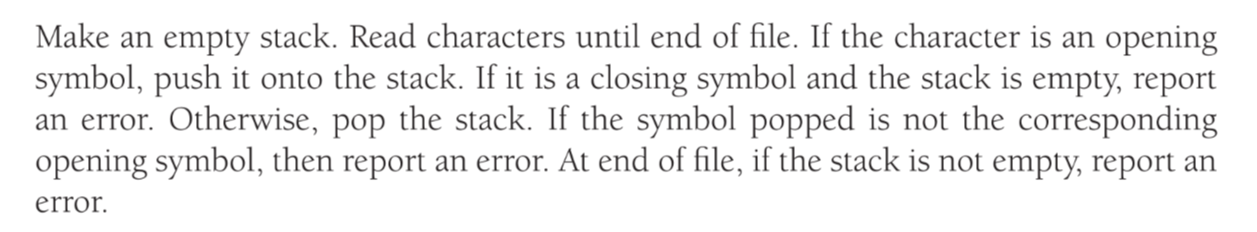
\includegraphics[width=1\textwidth]{img/Problema1Solucion.png}
  \end{figure}

\end{frame}


\begin{frame}
  \frametitle{Pasos}
  \begin{figure}[h]
    \centering
    
\includegraphics[width=0.6\textwidth]{img/Problema1-1.png}
  \end{figure}
\end{frame}

\begin{frame}
  \frametitle{Pasos}

  \begin{columns}
    \begin{column}{.5\textwidth}
  \begin{figure}[h]
    \centering
    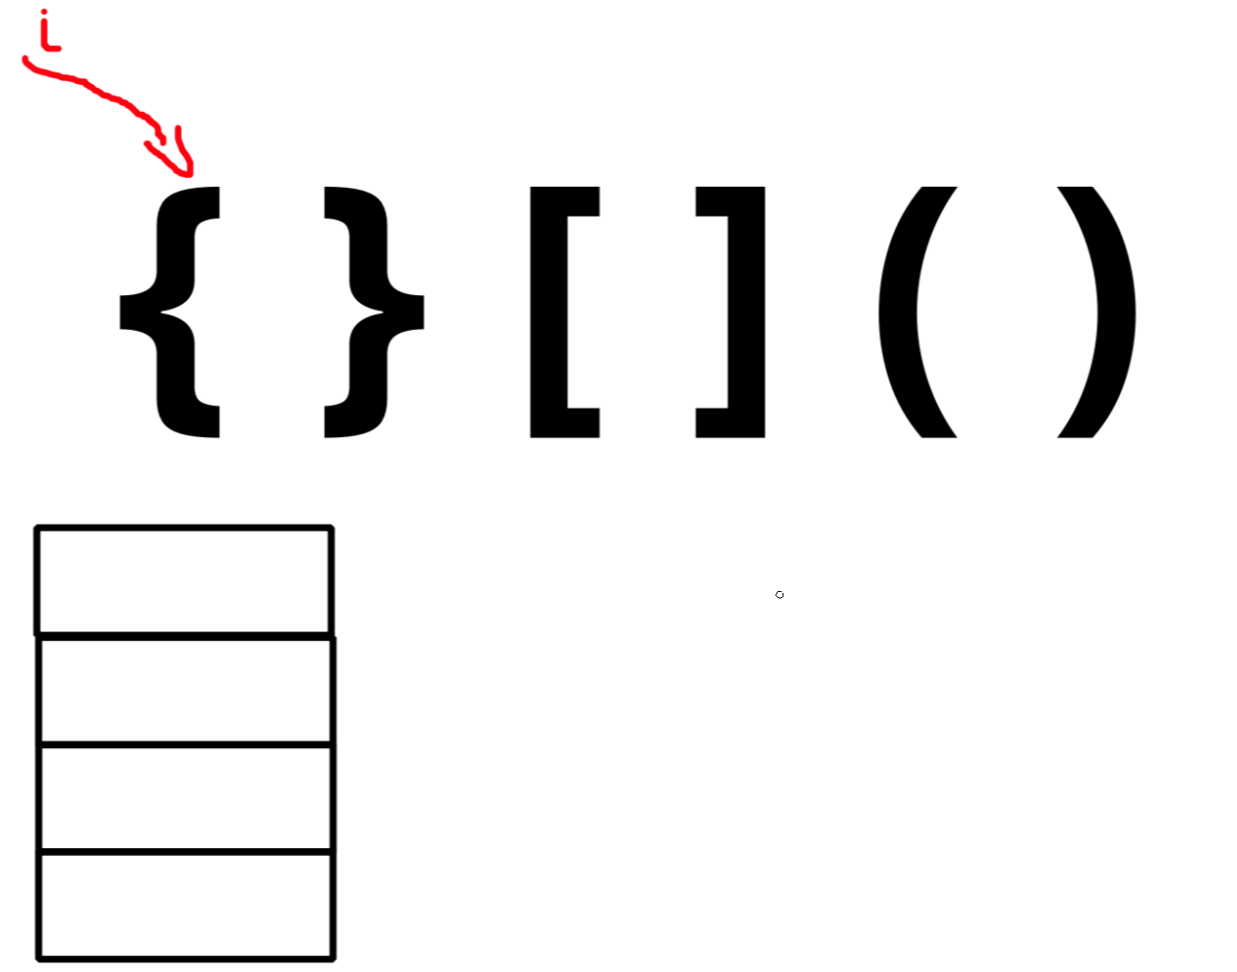
\includegraphics[width=0.8\textwidth]{img/Problema1-2.png}
  \end{figure}
    \end{column}

    \begin{column}{.5\textwidth}
      \begin{itemize}
        \item ¿Es $i$ un símbolo abierto?
        \item Sí, mover al \textit{stack}.
      \end{itemize}
    \end{column}
  \end{columns}

\end{frame}

\begin{frame}
  \frametitle{Pasos}
  \begin{figure}[h]
    \centering
    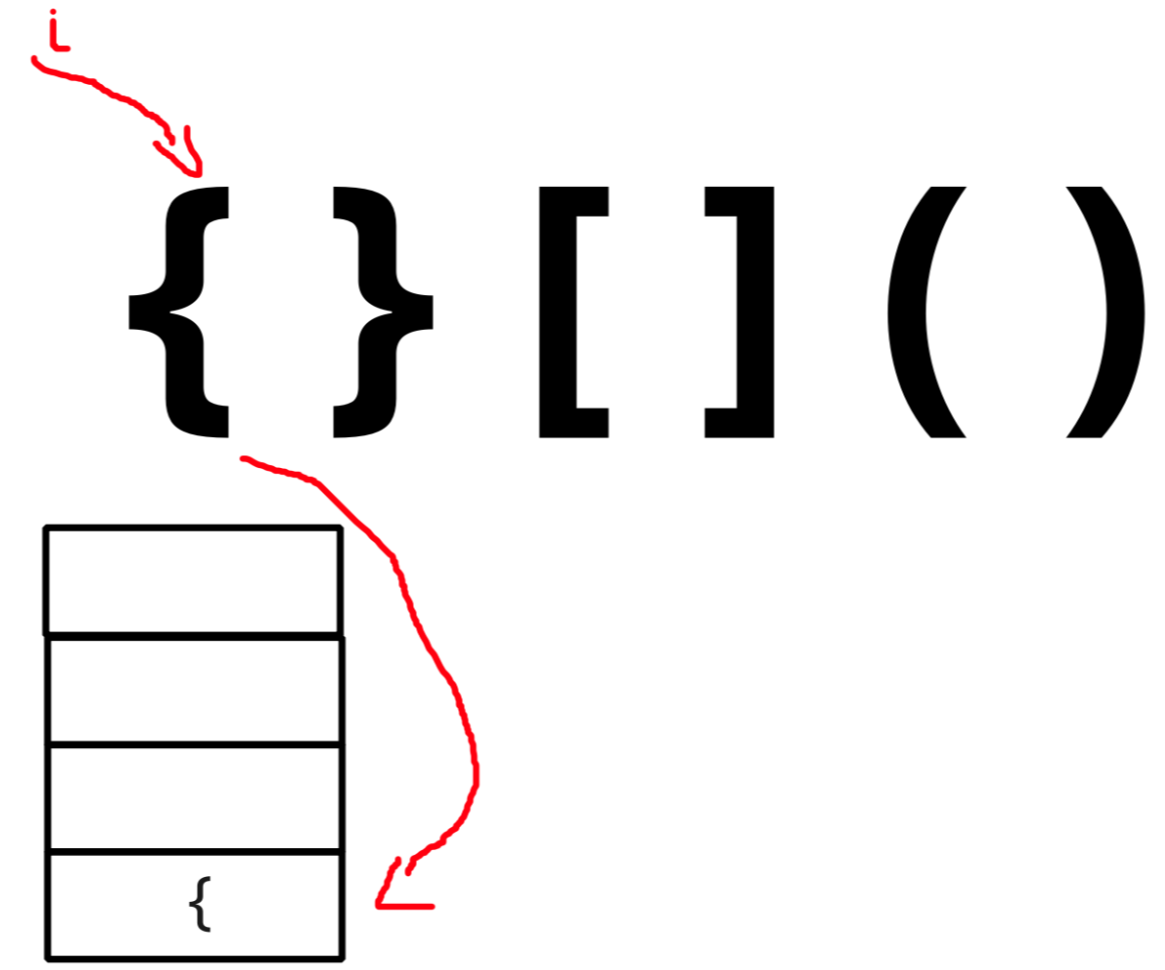
\includegraphics[width=0.5\textwidth]{img/Problema1-3.png}
  \end{figure}
\end{frame}

\begin{frame}
  \frametitle{Pasos}

  \begin{columns}
    \begin{column}{.5\textwidth}
  \begin{figure}[h]
    \centering
    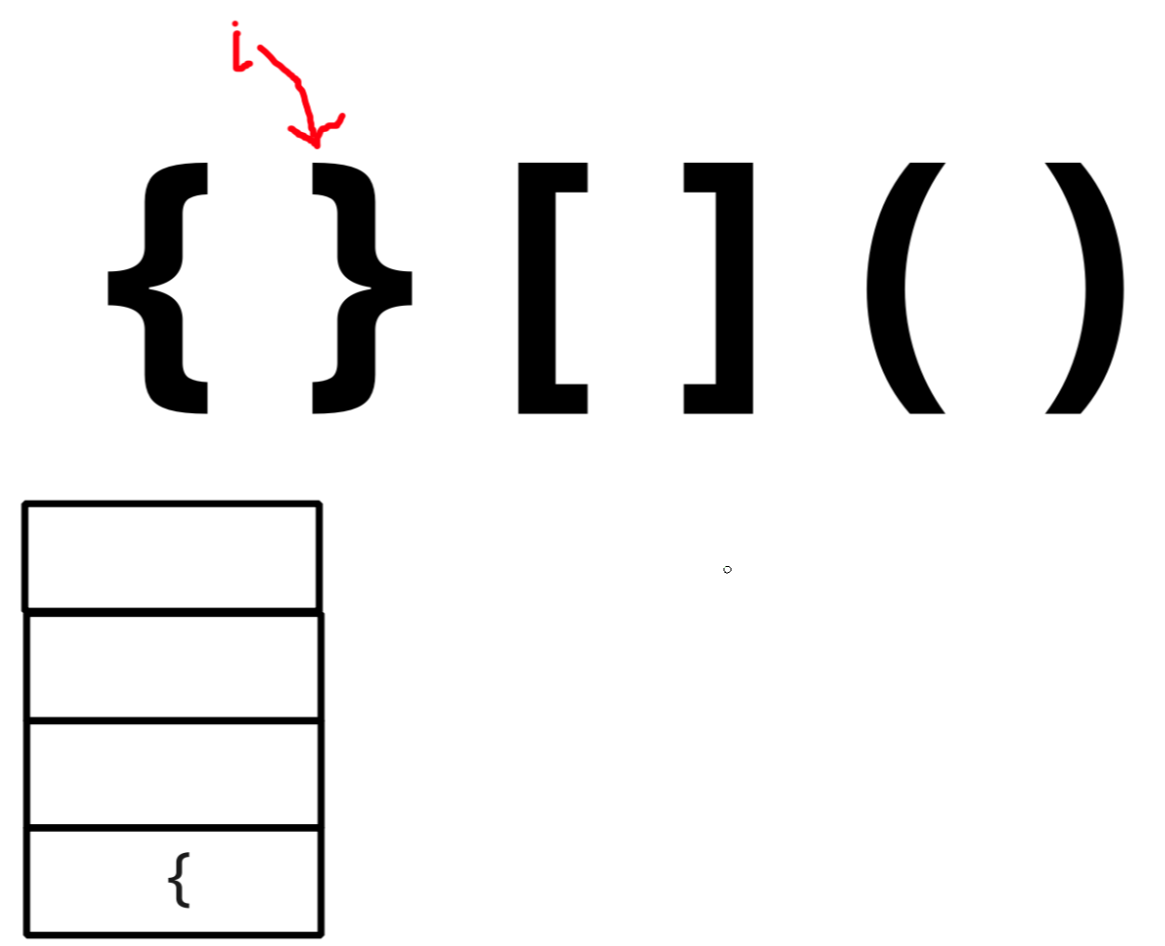
\includegraphics[width=0.8\textwidth]{img/Problema1-4.png}
  \end{figure}
    \end{column}

    \begin{column}{.5\textwidth}
      \begin{itemize}
        \item ¿Es $i$ símbolo cerrado?
        \item Sí, ¿Está vacía la cola?
        \item No, hacer \cppinline{pop} al \textit{stack}
      \end{itemize}
    \end{column}
  \end{columns}

\end{frame}

\begin{frame}
  \frametitle{Pasos}
  \begin{figure}[h]
    \centering
    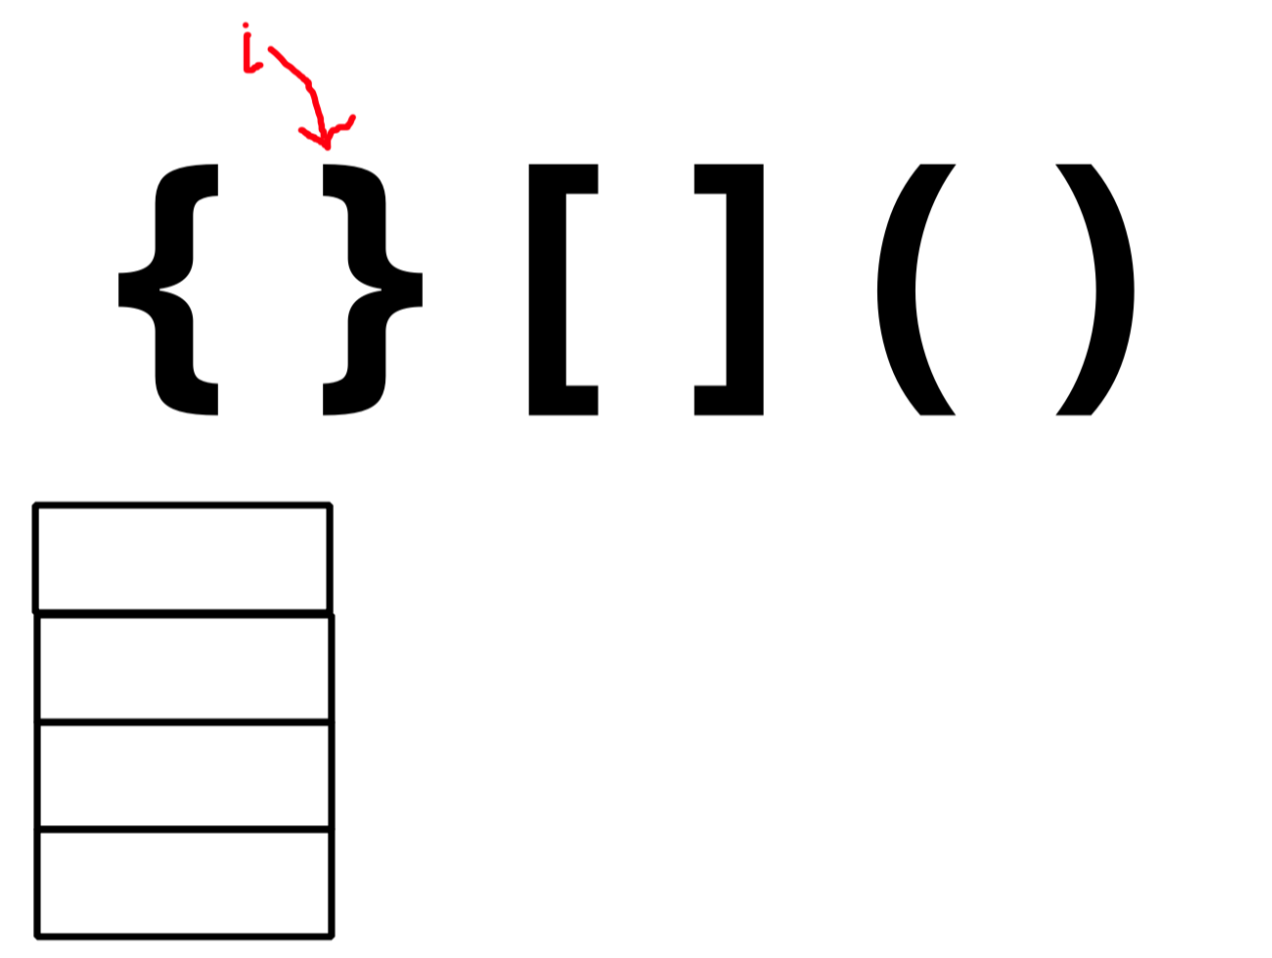
\includegraphics[width=0.5\textwidth]{img/Problema1-5.png}
  \end{figure}
\end{frame}




\begin{frame}
  \frametitle{Pasos}

  \begin{columns}
    \begin{column}{.5\textwidth}
  \begin{figure}[h]
    \centering
    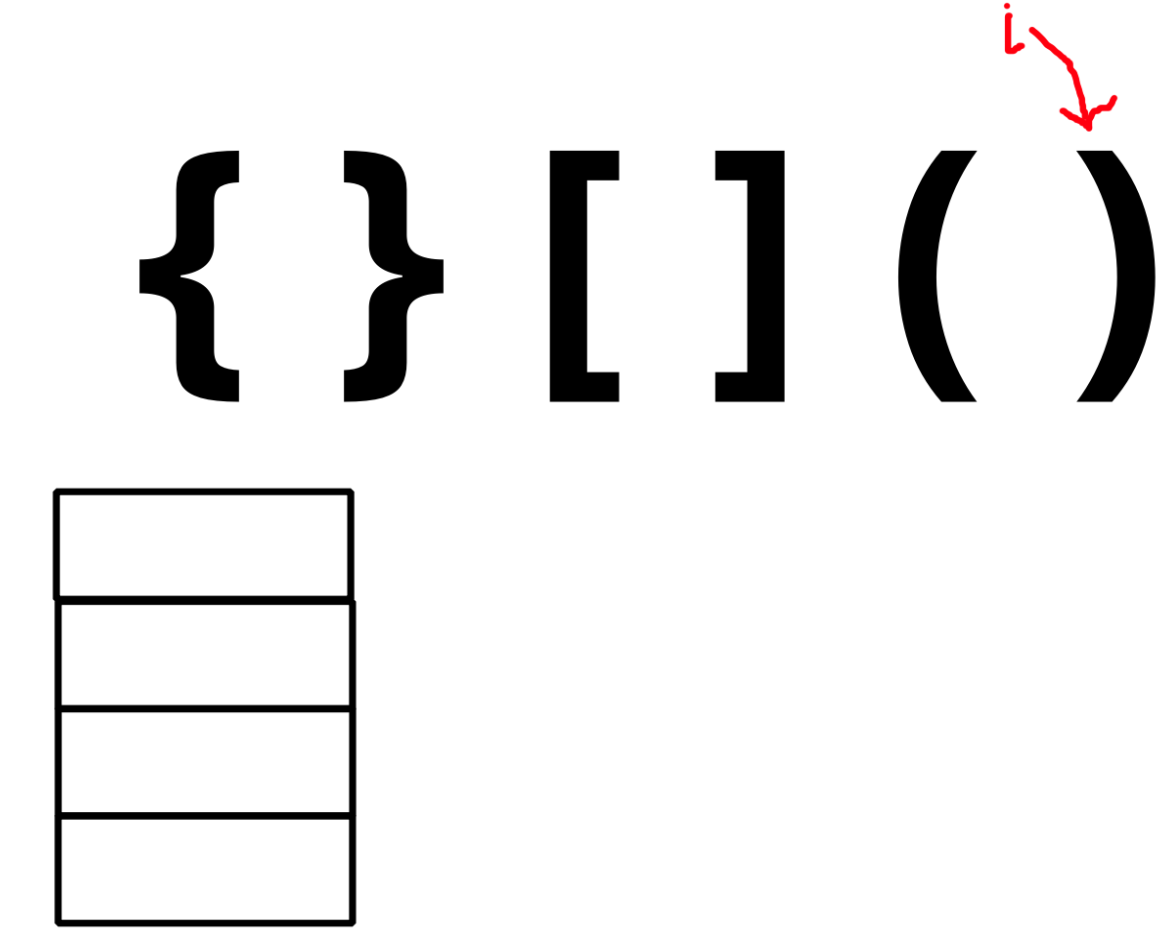
\includegraphics[width=0.8\textwidth]{img/Problema1-6.png}
  \end{figure}
    \end{column}

    \begin{column}{.5\textwidth}
      \begin{itemize}
        \item ¿Está el \textit{stack} vacío?
        \item Sí, devolver \cppinline{True}.
      \end{itemize}
    \end{column}
  \end{columns}

\end{frame}

\section{Diagrama de flujo}

\insertsectionpage

\begin{frame}
  \frametitle{Diagrama de flujo}
  \begin{figure}[h]
    \centering
    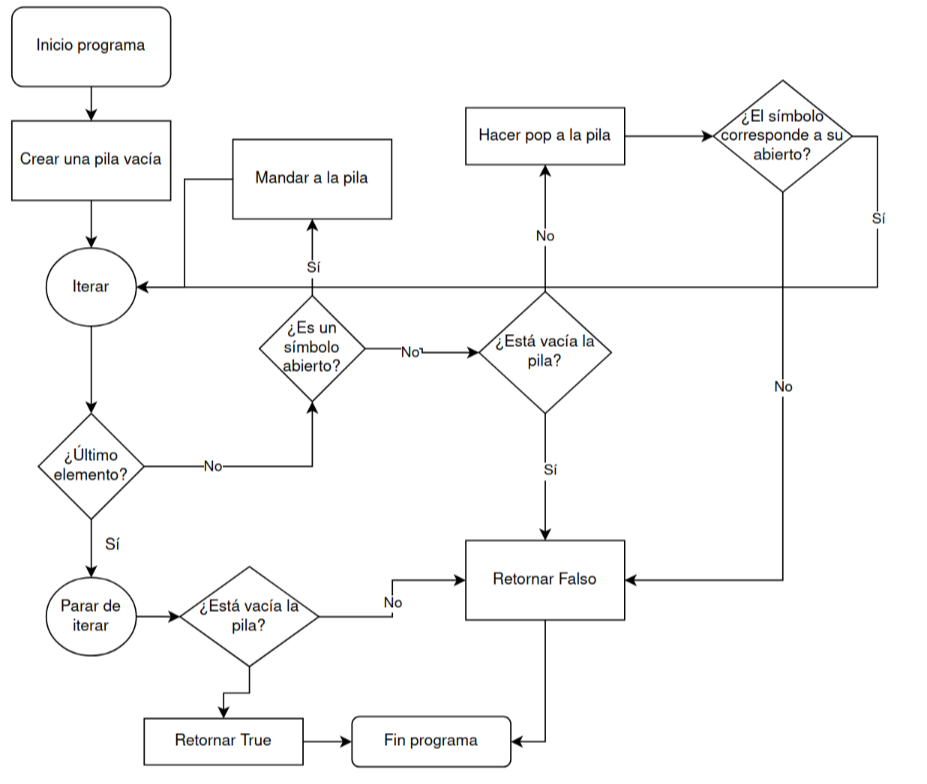
\includegraphics[width=0.5\textwidth]{img/Problema1-7.png}
  \end{figure}
\end{frame}


\section{Implementación En C++}

\insertsectionpage

\begin{frame}
  \frametitle{Implementación en C++}

 \scalebox{0.4}{\lstinputlisting[style=cppstyle]{Problema1.cpp}}

\end{frame}

\section{Complejidad temporal y espacial}

\insertsectionpage

\begin{frame}
  \frametitle{Complejidad temporal y espacial}

  \begin{itemize}
    \item Temporal:
          \[O(n)\]
    \item Espacial:
          \[O(n)\]
  \end{itemize}

\end{frame}








\section{Referencias}

\insertsectionpage
\begin{frame}[allowframebreaks]{Referencias}
  \printbibliography
\end{frame}


\insertendpage

\end{document}
